\chapter{Developer Documentation}
\label{developer-documentation}

\section{System Design}

\subsection{Detailed Problem Specification}
The software engineering task involves developing a scalable, high-concurrency threat intelligence platform capable of ingesting diverse modalities (URL, email, text), orchestrating asynchronous analysis pipelines (DNS, WHOIS, NLP, Reputation), executing an ML inference engine, and returning a deterministically weighted threat score and explanation within strict latency constraints.

\subsection{Logical and Physical Structure}
\subsubsection{The Tech Stack}
The physical architecture of PhishGuard is built upon a modern, distributed full-stack paradigm:
\begin{itemize}
    \item \textbf{Frontend (Vercel):} The user interface is implemented using Next.js (React) and TypeScript, deployed globally on Vercel's Edge Network for optimal performance and CDN caching.
    \item \textbf{Backend (Render):} The analysis engine and REST API are built with Python FastAPI, containerized via Docker, and deployed on Render to handle CPU-intensive ML inferences and asynchronous I/O operations.
    \item \textbf{Version Control (GitHub):} The entire source code, issue tracking, and CI/CD pipelines are managed via GitHub repositories.
\end{itemize}

\subsection{Architectural Overview}\label{architectural-overview}

The PhishGuard platform is engineered as a modern, decoupled, full-stack
web application. The architectural design prioritizes low-latency
inference, modular separation of concerns, and a seamless user
experience. To achieve these objectives, the system adopts a
client-server architecture, cleanly separating the user interface and
presentation logic from the heavy computational requirements of the
machine learning and Open-Source Intelligence (OSINT) pipelines.

The overarching architecture is composed of two primary subsystems: 1.
\textbf{The Client-Side Application (Frontend):} A responsive web
interface built with Next.js 16 and React 19. It is responsible for
accepting user input, rendering complex analytical visualizations, and
managing client-side state. 2. \textbf{The Analytical Engine (Backend):}
A high-performance, asynchronous REST API constructed using the FastAPI
framework in Python. It orchestrates the Natural Language Processing
(NLP) pipeline, executes asynchronous network OSINT queries, performs
feature engineering, and serves the XGBoost machine learning model.

This separation of concerns ensures that computationally expensive
operations---such as executing concurrent DNS queries and traversing
gradient-boosted decision trees---do not block the main thread of the
user interface, thereby guaranteeing a fluid and responsive user
experience even under heavy analytical load.

\subsection{High-Level Data Flow}\label{high-level-data-flow}

The operational lifecycle of a threat analysis request within the
PhishGuard architecture follows a deterministic, multi-stage pipeline.
The data flow is designed to dynamically adapt based on the modality of
the input (URL, email, or unstructured text).

\begin{figure}
\centering
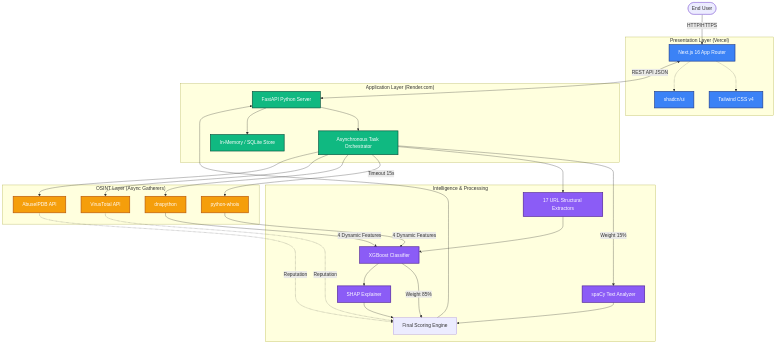
\includegraphics[width=0.85\linewidth,height=0.65\textheight,keepaspectratio]{images/system-architecture.png}
\caption{High-Level System Data Flow separating the Next.js
Presentation layer, FastAPI Application Orchestrator, ML Pipeline, and
Async OSINT}
\end{figure}

\subsection{Input Modality
Detection}\label{input-modality-detection}

Upon receiving a payload from the client via the \texttt{/api/analyze}
endpoint, the backend orchestrator first subjects the input to a
heuristic classification layer to determine its fundamental nature. The
\texttt{\_detectContentType} method in \texttt{orchestrator.py} utilizes
rigorous regular expressions and parsing logic to classify the input
into one of three categories: - \textbf{URL:} Detected if the string
begins with protocol identifiers (\texttt{http://}, \texttt{https://})
or matches a strict bare-domain regular expression pattern (e.g.,
\texttt{google.com}). - \textbf{Email:} Detected if the text block
contains standard RFC 5322 email headers, specifically checking for the
presence of substrings such as ``from:'', ``subject:'', and ``to:''. -
\textbf{Free Text:} Any unstructured text that fails to meet the strict
criteria of a URL or email header defaults to generic text analysis.

This dynamic, ``auto'' detection allows the user to paste any suspicious
content into a single, unified input field without needing to manually
specify the content type, significantly reducing user friction. Once the
modality is determined, the \texttt{\_extractDomain} method leverages
\texttt{urllib.parse} and custom regex to isolate the base domain, which
is a prerequisite for subsequent OSINT lookups.

\subsection{Asynchronous OSINT
Orchestration}\label{asynchronous-osint-orchestration}

\begin{figure}
\centering
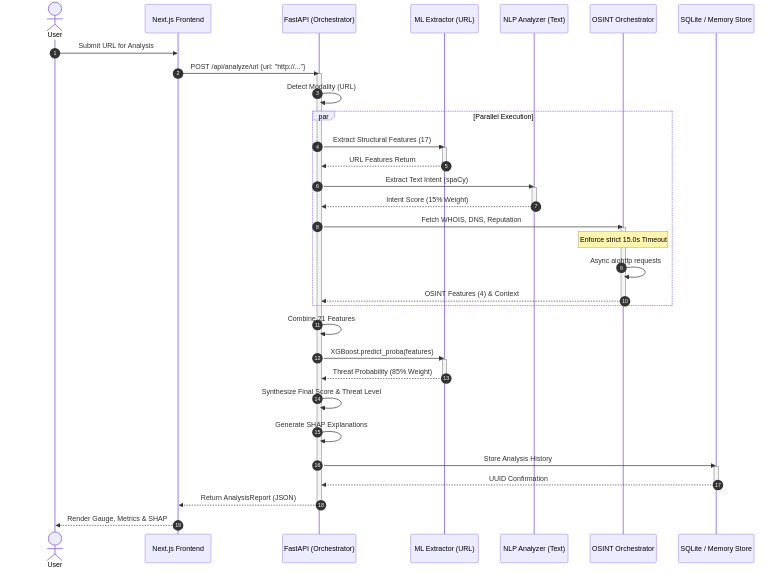
\includegraphics[width=0.85\linewidth,height=0.65\textheight,keepaspectratio]{images/sequence-diagram.png}
\caption{Sequence Diagram illustrating parallel execution of
Structural Features, NLP Analysis, and the strict 15.0s OSINT timeout}
\end{figure}

The integration of real-time OSINT constitutes the primary bottleneck in
the analysis pipeline. Querying global DNS servers, establishing WHOIS
connections, and communicating with third-party threat intelligence APIs
introduce unavoidable network latency.

To mitigate this, the FastAPI backend heavily leverages Python's
\texttt{asyncio} ecosystem. Within the \texttt{\_collectOsintData}
method, the system does not execute these external queries sequentially.
Instead, it utilizes \texttt{asyncio.gather} to concurrently execute
\texttt{lookupWhois(domain)}, \texttt{lookupDns(domain)}, and
\texttt{lookupReputation(domain)}.

Crucially, this parallel execution is wrapped in an
\texttt{asyncio.wait\_for} block with a strict global timeout of 15.0
seconds. This architectural safeguard ensures that unresponsive external
servers or rate-limited third-party APIs do not cause the internal event
loop to hang indefinitely. The system is designed to fail gracefully; if
an OSINT query times out or returns an exception, the orchestrator
catches it, logs the failure, and proceeds with the analysis utilizing
the available subset of data (or falling back to pure ML/NLP
heuristics).

\section{The API and Scoring
Engine}\label{the-api-and-scoring-engine}

\subsection{Weighted Verdict
Combination}\label{weighted-verdict-combination}

The core intelligence of the system resides in how the
\texttt{AnalysisOrchestrator} synthesizes disparate analytical signals
into a singular, actionable verdict. Because the system supports
multi-modal inputs, the scoring logic must dynamically adjust the
mathematical weight of each component based on the input type.

The \texttt{\_combineVerdict} method implements the following weighting
algorithm:

\textbf{For URL Inputs:} When the input is a URL, the XGBoost model is
treated as the supreme authority because its training data implicitly
encoded both lexical and OSINT features. - \textbf{Machine Learning
(XGBoost):} 85\% (\texttt{ML\_PRIMARY\_WEIGHT}) - \textbf{NLP Text
Analysis:} 15\% (\texttt{TEXT\_SUPPLEMENT\_WEIGHT})

\textbf{For Email/Text Inputs:} When analyzing raw text or emails, the
raw lexical URL features become secondary to the semantic meaning of the
content. - \textbf{NLP Text Analysis:} 55\%
(\texttt{TEXT\_PRIMARY\_WEIGHT}) - \textbf{URL Lexical Features
(Extracted from text):} 25\% (\texttt{URL\_SECONDARY\_WEIGHT}) -
\textbf{OSINT Infrastructure Score:} 20\%
(\texttt{OSINT\_SECONDARY\_WEIGHT})

The resulting aggregate score is bounded between 0.0 and 1.0. This score
is then mapped to definitive threat levels: - \textbf{Safe:} Score
$<${} 0.3 (\texttt{THREAT\_SAFE\_UPPER}) - \textbf{Suspicious:}
Score $<${} 0.5 (\texttt{THREAT\_SUSPICIOUS\_UPPER}) -
\textbf{Dangerous:} Score $<${} 0.7
(\texttt{THREAT\_DANGEROUS\_UPPER}) - \textbf{Critical:} Score \(\ge\)
0.7

This tiered approach allows the frontend to render appropriate visual
warnings and dynamic recommendations (e.g., ``Do not click links or
provide information'' for `Dangerous' classifications).

\subsection{Ephemeral History
Store}\label{ephemeral-history-store}

Consistent with the project's scope as a lightweight, deployable
prototype, PhishGuard eschews the architectural complexity of a
persistent relational database (e.g., PostgreSQL or MySQL). Instead, the
backend implements a highly efficient, thread-safe, in-memory
\texttt{HistoryStore} located in \texttt{backend/api/historyStore.py}.

The backend module utilizes a standard Python \texttt{collections.deque}
structured as a First-In-First-Out (FIFO) queue with a hard limit of 100
entries (\texttt{MAX\_ENTRIES}) for internal logging purposes. However, the
user-facing history persistence is implemented in the frontend using the
browser's localStorage API, which respects the user's configurable maximum
entry limit (10, 25, 50, or 100 entries as specified in the Settings page).
When a user submits an analysis, both stores record the full
\texttt{AnalysisResponse} object with a unique UUID and precise timestamp.

Because FastAPI operates on a single primary event loop, concurrent
asynchronous mutations to the backend deque are fundamentally thread-safe
without requiring complex locking mechanisms (like
\texttt{asyncio.Lock}). This design allows users to review their recent
analysis history via paginated API calls instantly, without the latency,
scaling, or configuration overhead of a persistent database connection.

\subsection{Pydantic Schema
Contracts}\label{pydantic-schema-contracts}

\begin{figure}
\centering

\includegraphics[width=0.85\linewidth,height=0.65\textheight,keepaspectratio]{images/class-diagram.png}
\caption{UML Class Diagram defining the strict Pydantic data
contracts enforcing backend type safety}
\end{figure}

To guarantee structural integrity between the Next.js frontend and the
FastAPI backend, PhishGuard utilizes Pydantic models to define strict
data contracts. Every incoming request and outgoing response is
automatically validated, serialized, and documented via OpenAPI.

For example, the core \texttt{AnalysisResponse} schema mathematically
guarantees that the frontend will always receive a deterministic JSON
object. This object contains the \texttt{VerdictResult} (including the
boolean \texttt{isPhishing} flag and float \texttt{confidenceScore}),
the \texttt{OsintSummary}, and the \texttt{FeatureSummary}. This strict
validation eliminates runtime \texttt{TypeError} and \texttt{KeyError}
exceptions in the frontend UI, providing a robust, self-documenting API
contract.

\subsection{Frontend Architecture}\label{frontend-architecture}

The presentation layer is constructed using Next.js 16 (App Router) and
React 19, focusing heavily on performance, modern UI/UX paradigms, and
data visualization.

\subsection{Component-Based
Structure}\label{component-based-structure}

The user interface is strictly modular, adhering to React's
component-based philosophy. The architecture leverages the
\texttt{shadcn/ui} component library alongside \texttt{@base-ui/react}
to provide accessible, highly customizable foundational components
(e.g., buttons, input fields, modals).

The application logic is separated into logical directories: -
\texttt{src/app}: Contains the Next.js App Router logic, global layouts,
and top-level page components (such as the analyzer dashboard and
history views). - \texttt{src/components}: Houses reusable UI elements.
Complex visual representations, such as risk gauges or metric cards, are
isolated here.

\subsection{State Management and Client-Server
Interaction}\label{state-management-and-client-server-interaction}

State management within the application is handled primarily through
React's native hooks (\texttt{useState}, \texttt{useEffect}). The
application consciously avoids heavyweight global state managers (like
Redux or Zustand) in favor of localized, prop-drilled state where
appropriate. This architectural choice aligns with the modern Next.js
paradigm, which encourages keeping state as close to the UI components
as possible to minimize unnecessary re-renders.

Communication with the FastAPI backend is achieved via native
\texttt{fetch} requests. The application utilizes the \texttt{sonner}
library to provide non-blocking, toast-based notification feedback to
the user regarding the success or failure of network requests, ensuring
the user is always aware of the system's status during the 1-3 seconds
required for OSINT queries.

For results delivery, the frontend uses a layered restoration strategy.
The primary transfer path is an in-memory \texttt{ResultsContext} for
fast post-analysis navigation. For shareability and cross-session
reliability, the ``Copy Link'' action serializes the full
\texttt{AnalysisResponse} payload into a compact URL-safe query value
(\texttt{r}), optionally alongside a local history identifier
(\texttt{hid}). On page load, the Results route restores in order:
context \(\rightarrow\) query payload \(\rightarrow\) history lookup.
This guarantees that shared report links remain reproducible even in
private/incognito browser sessions.

\subsection{Visual Presentation and
Theming}\label{visual-presentation-and-theming}

A critical requirement of the system was the delivery of a professional,
``dark-mode'' optimized aesthetic typical of modern cybersecurity
platforms. The application achieves this via \texttt{tailwindcss}
(version 4) for utility-first styling and \texttt{next-themes} for
seamless theme switching.

The visual hierarchy utilizes distinct color coding to rapidly
communicate the threat levels computed by the backend orchestrator:
green for `Safe', amber for `Suspicious', and red for critical
`Phishing' indicators. Fluid animations and layout transitions, powered
by the \texttt{motion} library, are employed to provide immediate visual
feedback during the analysis lifecycle. The Analyse page progress
component is event-driven rather than timer-simulated, exposing concrete
frontend phases (preparing, sending, waiting, processing, complete)
plus elapsed time while the request is in-flight. This improves UX
honesty and makes the loading state auditable during manual QA.

\subsection{System Design Summary}\label{summary-1}

This chapter detailed the structural engineering of the PhishGuard
platform. The architecture successfully isolates the Next.js
presentation layer from the FastAPI analytical engine. By employing an
asynchronous concurrency model in Python (\texttt{asyncio.gather} with
global timeouts) and an in-memory \texttt{deque} for history management,
the system achieves the necessary performance metrics required for
real-time threat analysis. Furthermore, the orchestrator's dynamic
weighting algorithms ensure accurate assessments across diverse input
modalities.

The subsequent chapters, will delve deeply into the
mathematical core of this architecture: the feature engineering
pipeline, the XGBoost classification model, and the Optuna optimization
strategy.



\section{System Architecture and
Overview}\label{system-architecture-and-overview}

This section provides additional deployment context. The complete architectural design is detailed in Section \ref{architectural-overview}.

\begin{figure}[htbp]
\centering
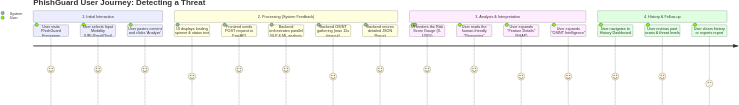
\includegraphics[width=\textwidth,keepaspectratio]{images/user-journey.png}
\caption{The End-to-End User Journey, illustrating the
transition from input submission to reviewing Explainable AI (SHAP)
metrics}
\end{figure}

The implementation uses FastAPI (Python) for the backend and Next.js 16 with React 19 for the frontend, as described in Section \ref{architectural-overview}.

\subsection{Backend Framework and
Initialization}\label{backend-framework-and-initialization}

FastAPI was selected as the foundational framework due to its native
support for asynchronous programming (\texttt{asyncio}), automatic
interactive API documentation generation (Swagger UI via OpenAPI), and
robust data validation utilizing Pydantic models.

The application entry point (\texttt{backend/main.py}) defines the
global state and configuration through the \texttt{lifespan} context
manager. This approach efficiently manages application startup and
shutdown events, logging the initialized configuration, analyzer engine
states, and Cross-Origin Resource Sharing (CORS) rules.

The CORS middleware is explicitly configured to ensure secure
communication between the frontend client and the backend API,
particularly when deployed in production environments. A strict warning
is logged if wildcard origins (\texttt{*}) are detected in production
(\texttt{settings.isProduction}), demonstrating a defense-in-depth
approach to application security.

Furthermore, custom exception handlers (\texttt{valueErrorHandler} and
\texttt{genericExceptionHandler}) are implemented to standardise error
responses. In debug mode, stack traces and detailed exception types are
exposed, whereas in production environments, generic internal server
error messages are returned to prevent information disclosure.


\subsection{The Analysis Orchestrator}\label{the-analysis-orchestrator}

The core computational logic of the application resides within the
\texttt{backend/api/orchestrator.py} module. This module coordinates the
various independent analysis pipelines: Open-Source Intelligence
(OSINT), Machine Learning (ML), and Natural Language Processing (NLP).

The orchestrator utilizes Python's asynchronous I/O capabilities
(\texttt{asyncio.gather}) to concurrently execute independent tasks.
This design is critical for performance; DNS queries, WHOIS lookups, and
API calls to reputation services (e.g., VirusTotal, AbuseIPDB) are
inherently bound by network latency rather than CPU constraints. By
executing these tasks concurrently rather than sequentially, the total
response time is bounded by the slowest individual external service
rather than the sum of all their latencies.

The orchestrator aggregates the results from the \texttt{OsintData},
\texttt{NlpAnalyzer}, and the \texttt{PhishingPredictor} components into
a unified \texttt{AnalysisResponse} object. This response structure
provides the frontend client with a holistic view of the analyzed
entity, including discrete categorical scores, confidence metrics, and
human-readable explanation factors.


\section{Production Hardening: Endpoint Security, Observability, and Resilient Monitoring}\label{production-hardening}

A detection system that surfaces ``no threat detected'' for an analysed phishing URL is not the same as a detection system that survives the next six months in production. Beyond the analysis pipeline itself, PhishGuard ships a defence-in-depth posture that protects the API surface, throttles abuse, authenticates callers, emits machine-readable logs, and gives uptime monitors an honest view of dependency health. The following five middleware and module components compose this hardening posture.

\subsection{HTTP Security Headers (OWASP Baseline)}

Following the OWASP Secure Headers Project recommendations, every outgoing response is augmented with hardened HTTP headers through the \texttt{backend/api/security\_headers.py} module, registered as a Starlette HTTP middleware in \texttt{main.py}.

\begin{itemize}
\item
  \texttt{X-Content-Type-Options:\ nosniff} -- prevents MIME-confusion attacks in browsers; forces \texttt{application/json} to be treated as \texttt{application/json}.
\item
  \texttt{X-Frame-Options:\ DENY} together with CSP \texttt{frame-ancestors\ 'none'} -- disallows any iframe embedding, mitigating clickjacking against the Swagger UI surface.
\item
  \texttt{Referrer-Policy:\ strict-origin-when-cross-origin} -- sends only the origin on cross-origin navigation; prevents URL leakage to third parties.
\item
  \texttt{Content-Security-Policy:\ default-src\ 'none';\ frame-ancestors\ 'none';\ base-uri\ 'none';\ form-action\ 'none'} -- the most conservative CSP that is compatible with FastAPI's Swagger UI; the docs path is the only place where inline scripts and CDN-loaded styles are permitted.
\item
  \texttt{Strict-Transport-Security:\ max-age=31536000;\ includeSubDomains} -- emitted only in production; local development over plain HTTP does not benefit from HSTS and some local proxies misinterpret it.
\end{itemize}

The middleware binds the production-mode boolean at registration time rather than reading the live \texttt{settings} object inside the closure. This avoids timing-sensitive behaviour of \texttt{pydantic-settings}' \texttt{lru\_cache} during pytest runs where the environment toggles between tests; the production-mode header decisions are made once, deterministically.

\subsection{Rate Limiting via \texttt{slowapi}}

Public OSINT queries cost the system real third-party API quota, and unbounded traffic from a single scraper would burn the budget for legitimate users. The \texttt{backend/api/rate\_limiting.py} module introduces per-key rate budgets via the \texttt{slowapi} library:

\begin{itemize}
\item
  Per-IP default: 60 requests per minute -- covers routes that do not carry an explicit \texttt{@limiter.limit} decorator such as \texttt{/api/health} and \texttt{/api/history*}.
\item
  Heavy analysis routes (\texttt{/api/analyze}, \texttt{/api/analyze/url}, \texttt{/api/analyze/email}): 30 requests per minute per IP -- each call burns WHOIS, VirusTotal, AbuseIPDB, and XGBoost inference budget.
\item
  \texttt{/api/model/status}: 10 requests per minute -- this is a cheap inspection endpoint and does not need a generous budget.
\end{itemize}

The slowapi key function prefers \texttt{X-Api-Key} headers over \texttt{X-Forwarded-For} chains over the raw remote address. An authenticated caller therefore gets one bucket per API key regardless of which network they connect from, preventing an adversary with a rotating residential proxy from exceeding the budget.

The slowapi exception handler is overridden so that the standard plaintext 429 is replaced with a JSON envelope:

\begin{verbatim}
{
  "detail": "Rate limit exceeded",
  "limit": "30 per 1 minute",
  "retry_after_seconds": 60
}
\end{verbatim}

\texttt{slowapi} supports multiple storage backends. The in-process \texttt{memory://} backend is appropriate for the Render free plan's single-instance topology; production multi-instance deployments can opt into Redis-backed storage by setting \texttt{PHISHGUARD\_RATE\_LIMIT\_URI=redis://...}.

\subsection{Optional X-Api-Key Authentication}

Authentication is the third leg of the defence-in-depth posture. The \texttt{backend/api/auth.py} module registers a middleware that gates the heavy \texttt{/api/analyze*} routes behind an \texttt{X-Api-Key} shared secret. The key list is configured via the \texttt{APIKEYS} environment variable as a comma-separated list.

The implementation has three important properties:

\begin{enumerate}
\item
  Configured keys are immediately digested into SHA-256 hex digests at startup; raw key bytes never sit in process memory during operation.
\item
  Each incoming key is hashed before comparison, and the digest is matched against the configured set with \texttt{hmac.compare\_digest}, closing the timing-attack window that a naive \texttt{in} test would leave open.
\item
  Authentication runs before the rate-limit middleware, so an attacker spamming bad keys short-circuits at 401 and never consumes a rate-budget slot.
\end{enumerate}

When \texttt{APIKEYS} is unset, the middleware is registered but behaves as a pass-through; this preserves the current public-demo posture and lets operators tighten access by setting one env var. Failures generate a 401 response carrying both a JSON body and a \texttt{WW-Authenticate:\ ApiKey} response header per RFC-7235. Auth is a single decision so the entire route handler short-circuits the rest of the middleware chain.

\subsection{Structured Logging and Request Correlation}

Operational observability is the fourth leg. \texttt{backend/logging\_config.py} replaces the default Python \texttt{logging} formatter with a \texttt{structlog} processor pipeline:

\begin{itemize}
\item
  Production (\texttt{LOG\_FORMAT=json} or the production environment flag): one JSON object per line, ISO-8601 UTC timestamps, suitable for log aggregators such as Render's built-in log explorer.
\item
  Development / testing: colourised console output (\texttt{structlog.dev.ConsoleRenderer}) for human readability on the operator's terminal.
\item
  Standard-library \texttt{logging.getLogger(\_\_name\_\_)} call sites are bridged through the same processor chain via \texttt{ProcessorFormatter}, so existing code requires no refactor and still emits structured records.
\end{itemize}

A second middleware (\texttt{\_RequestIdMiddleware}) ensures every incoming request carries an \texttt{X-Request-ID} header -- either echoed from the client or generated as a 12-character hex value -- and binds the id into structlog's \texttt{contextvars}. Every log line emitted during that request therefore carries \texttt{request\_id=...} automatically, making post-mortem searches on an aggregation platform a single field-target operation.

The middleware is registered as the outermost layer in \texttt{main.py}, so an operator inspecting a 500-error log line can trace it back to the originating client by the \texttt{X-Request-ID} they were given in the error response.

\subsection{Deep Health Check for Uptime Monitors}

A shallow ``\texttt{/api/health} returns 200'' check lies to an uptime monitor when DNS has stopped resolving or when the XGBoost model silently failed to load. The \texttt{backend/health.py} module replaces the legacy handler with a deep probe that exercises every production-critical dependency in parallel:

\begin{itemize}
\item
  \textbf{DNS} -- resolve \texttt{example.com} via \texttt{backend.osint.dnsChecker.DnsChecker}; 3-second bounded timeout prevents a wedged resolver from starving the uptime endpoint.
\item
  \textbf{ML} -- instantiate \texttt{PhishingPredictor} and assert \texttt{isLoaded} is \texttt{True}; reports the number of features available to the scoring engine.
\item
  \textbf{Imports} -- re-import the analyser and orchestrator modules as a fast-fail sentinel against environment drift.
\end{itemize}

The three checks run via \texttt{asyncio.gather} so the slowest check (typically the DNS probe) bounds the latency \emph{and} the aggregated endpoint returns within 100--300 milliseconds even on slower connections. Per-check results carry a \texttt{status}, \texttt{latencyMs}, and a human-readable \texttt{detail}; the top-level \texttt{status} collapses to \texttt{healthy} (all checks \texttt{up}), \texttt{degraded} (DNS down but ML/imports up; OSINT queries will gracefully fail individually), or \texttt{unhealthy} (ML or imports down; URL phishing scoring cannot work). HTTP 503 is returned only on \texttt{unhealthy}; the \texttt{degraded} state returns 200 so uptime dashboards see OK but the inspection payload flags the situation. A backward-compatible \texttt{services} key (\texttt{osint}, \texttt{analyzer}, \texttt{ml}) is preserved for the existing client agents and dashboards that read it.

\subsubsection{Liveness / Readiness Probe Split (Kubernetes Semantics)} A naive \texttt{/api/health} endpoint conflates two very different questions, \emph{``is the process alive?''} and \emph{``is the system ready to serve production traffic?''}. The probes must be split because they have very different cost profiles: Render scans the liveness probe every second but the readiness probe only every ten seconds, and a slow readiness endpoint (DNS + ML probes each take hundreds of milliseconds) starves the liveness budget. Two endpoints are therefore exposed, both registered by \texttt{registerHealthEndpoints()} in \texttt{backend/health.py} and mounted under a shared \texttt{APIRouter} with the \texttt{/api/health} prefix:

\begin{itemize}
\item
  \texttt{GET /api/health/live} returns 200 in well under fifty milliseconds whenever the FastAPI event loop is alive; it performs no I/O, no probes, no module imports beyond what was required at startup. \texttt{render.yaml} points \texttt{healthCheckPath} at this endpoint so Render's per-second scans never burn the readiness budget.
\item
  \texttt{GET /api/health/ready} returns the deep probe envelope (\texttt{status}, \texttt{checks}, \texttt{services}, \texttt{uptimeSeconds}, \texttt{version}). This is what the load balancer should poll when deciding whether to route traffic to a new instance.
\item
  \texttt{GET /api/health} is kept as a permanent alias of \texttt{/ready} so external dashboards and existing scripts that hard-coded the path keep working unchanged.
\end{itemize}

\subsection{Hardening Test Surface}

The five hardening features are covered by 158 new pytest tests: 92 unit tests spanning the helper utilities (digest computation, key parser, formatter helpers, processor chains, aggregation logic, liveness vs readiness split, registerHealthEndpoints idempotence) and 66 integration tests covering the end-to-end FastAPI pipeline (header presence on every response, 401 and 429 status mapping, request-id header round-trip, deep health response shape, status-to-HTTP mapping, liveness latency budget, X-Request-ID across both probe paths). The full Tier 1 delivery brings the backend test count to 755 distinct pytest cases (with 12 additional long-pipeline integration tests that exercise the real orchestrator and are not included in the fast tier); all 743 fast tests complete in well under 90 seconds.

\section{Deployment and
Infrastructure}\label{deployment-and-infrastructure}

The PhishGuard application is designed for automated, seamless
deployment using a continuous integration and continuous deployment
(CI/CD) pipeline integrated with the Render platform.

The infrastructure configuration is defined declaratively within the
\texttt{render.yaml} blueprint file. This file specifies the deployment
parameters for the backend service (\texttt{phishguard-api}), dictating
the runtime environment (Python), the specific geographic region
(Frankfurt), and the build and execution commands.

Crucially, the blueprint explicitly maps environment variables required
for the application's operation. While general configuration settings
like \texttt{ENVIRONMENT} and \texttt{PYTHON\_VERSION} (3.10.12) are
hardcoded in the blueprint, sensitive credentials such as
\texttt{VIRUSTOTAL\_API\_KEY}, \texttt{ABUSEIPDB\_API\_KEY}, and
\texttt{CORS\_ORIGINS} are marked with \texttt{sync:\ false}. This
security measure ensures that API keys and proprietary configuration
details are strictly managed within the Render dashboard's secure
environment variable vault and are never committed to version control.

The application initiates via the Uvicorn ASGI web server, binding to
the port dynamically assigned by the Render platform environment
(\texttt{-\/-port\ \$PORT}). The health check endpoint
(\texttt{/api/health}) provides continuous monitoring capabilities,
allowing the load balancer to automatically route traffic away from
degraded instances, ensuring high availability.


\section{Integration and Weighting
Mechanisms}\label{integration-and-weighting-mechanisms}

The most critical function of the Analysis Orchestrator is to
algorithmically synthesize the discrete analytical outputs from the
OSINT, ML, and NLP modules into a singular, high-confidence verdict.
This synthesis is governed by a strict set of predefined weighting
constants designed to prioritize the most reliable signals based on the
input content type.

\subsection{The 15-Second Concurrency
Window}\label{the-15-second-concurrency-window}

The API enforces a strict 15-second timeout on all OSINT queries using \texttt{asyncio.wait\_for}. This prevents external service delays from blocking the response. The implementation details are described in Section \ref{asynchronous-osint-orchestration}.

\subsection{Content-Specific Scoring
Pipelines}\label{content-specific-scoring-pipelines}

The scoring algorithm dynamically adjusts weights based on input type. The exact implementation (85/15 for URLs, 55/25/20 for text) is detailed in Section \ref{weighted-verdict-combination}. This ensures the most reliable signal receives primary weight for each content type.

\subsection{The Phishing Threshold and Threat
Boundaries}\label{the-phishing-threshold-and-threat-boundaries}

The threat level boundaries (Safe < 0.3, Suspicious < 0.5, Dangerous < 0.7, Critical $\geq$ 0.7) are defined in Section \ref{weighted-verdict-combination}. These drive the color-coded UI recommendations shown to users.

\section{Quality Assurance and Testing}

\subsection{Testing Plan and Results}

In the domain of cybersecurity and threat intelligence, software
reliability is paramount. A false positive in a phishing detection
system can disrupt legitimate business operations, while a false
negative can result in severe data breaches. To mitigate these risks and
ensure the stability of the PhishGuard platform, a comprehensive,
multi-tiered Quality Assurance (QA) framework was implemented.

This framework strictly adheres to the principles of the software
testing pyramid, encompassing static analysis, isolated unit testing,
component integration testing, and end-to-end (E2E) browser automation.
The testing architecture is physically and logically partitioned to
mirror the application's microservice design, utilizing domain-specific
tooling for the Python-based API backend and the TypeScript-based
Next.js frontend.

\subsubsection{Backend Testing
Methodology}\label{backend-testing-methodology}

The backend testing architecture is constructed upon the \texttt{pytest}
framework, comprising 916 distinct tests (755 backend \texttt{pytest} unit/integration tests, 133 frontend \texttt{Jest} tests, and 28 \texttt{Playwright} E2E browser tests) distributed
across the \texttt{tests/unit/} and \texttt{tests/integration/}
directories. Given the asynchronous nature of the FastAPI orchestrator
and the underlying Open-Source Intelligence (OSINT) network calls, the
\texttt{pytest-asyncio} plugin is heavily utilized, configured centrally
via \texttt{pytest.ini} (\texttt{asyncio\_mode\ =\ auto}) to natively
resolve coroutines during test execution.

\paragraph{Environment Isolation and Fixture
Management}\label{environment-isolation-and-fixture-management}

To guarantee deterministic test execution and prevent state leakage
between discrete test cases, a robust fixture management system is
defined within \texttt{tests/conftest.py}. The framework enforces strict
environmental isolation utilizing the \texttt{pytest}
\texttt{monkeypatch} utility. The \texttt{isolatedEnvironment} fixture
automatically intercepts the execution context prior to each test,
forcibly overriding critical environment variables (e.g., setting
\texttt{ENVIRONMENT} to \texttt{testing} and \texttt{LOG\_LEVEL} to
\texttt{DEBUG}) and invoking \texttt{getSettings.cache\_clear()} to
purge any memoized configuration states.

\paragraph{Dependency Inversion and OSINT
Mocking}\label{dependency-inversion-and-osint-mocking}

The backend relies heavily on external, rate-limited threat intelligence
services (e.g., VirusTotal, WHOIS databases). Executing live network
requests during automated testing introduces severe latency,
unpredictable failures, and potential API quota exhaustion. To resolve
this, the QA architecture employs extensive dependency inversion and
mocking methodologies utilizing \texttt{unittest.mock.MagicMock} and
\texttt{AsyncMock}.

The \texttt{conftest.py} file exposes a suite of deterministic data
fixtures, such as \texttt{sampleWhoisData},
\texttt{suspiciousWhoisData}, and \texttt{privacyProtectedWhoisData}.
These dictionaries simulate the exact JSON payloads returned by
downstream services. Mock clients, such as
\texttt{mockWhoisClientTimeout}, intentionally inject
\texttt{asyncio.TimeoutError} exceptions into the pipeline, allowing the
test suite to mathematically verify the orchestrator's error handling
and fallback heuristics without relying on actual network degradation.

\subsubsection{Integration and Smoke
Testing}\label{integration-and-smoke-testing}

While unit tests validate discrete algorithmic functions (e.g., URL
parsing logic within \texttt{test\_urlAnalyzer.py}), the integration
layer verifies the holistic interaction between the FastAPI routing
layer, the Machine Learning (ML) predictor, and the OSINT aggregation
modules.

The \texttt{tests/integration/test\_smoke.py} suite utilizes the FastAPI
\texttt{TestClient} to perform programmatic HTTP requests against the
application interface. This suite is critical for validating the
structural integrity of the JSON responses
(\texttt{TestResponseFormatConsistency}) and ensuring the API conforms
precisely to the OpenAPI schema specifications.

\paragraph{Service Level Agreement (SLA)
Validation}\label{service-level-agreement-sla-validation}

Performance degradation is a critical failure state for synchronous
security APIs. The integration suite implements explicit quantitative
assertions to enforce performance SLAs. The \texttt{TestPerformance}
class programmatically submits batches of heterogeneous data
(\texttt{SAMPLE\_URLS} and \texttt{SAMPLE\_EMAILS}) and records the
execution duration utilizing the \texttt{time} module.

The testing framework enforces a strict upper bound defined by the
\texttt{MAX\_SECONDS\_PER\_ANALYSIS\ =\ 5.0} constant. Any holistic
analysis---including ML inference, NLP parsing, and mocked OSINT
aggregation---that exceeds this threshold results in an immediate test
failure. Similarly, the \texttt{/api/health} endpoint is rigorously
asserted to respond in under \texttt{1.0} seconds, ensuring load
balancers can rapidly assess instance viability.

\subsubsection{Frontend Quality
Assurance}\label{frontend-quality-assurance}

The Next.js client application employs an orthogonal testing strategy
tailored to React component lifecycles and browser Document Object Model
(DOM) interactions.

\paragraph{Component and State
Validation}\label{component-and-state-validation}

Unit testing for the frontend is executed utilizing the \texttt{jest}
framework augmented by \texttt{@testing-library/react}. This layer
validates internal state management logic and isolated UI component
rendering. For example, test suites such as
\texttt{historyStore.test.ts} programmatically verify the application's
ability to serialize and deserialize historical analysis records to
local storage, while component tests ensure that risk indicators
strictly map to the correct visual paradigms defined by Tailwind CSS
utility classes.

\paragraph{End-to-End (E2E) Browser
Automation}\label{end-to-end-e2e-browser-automation}

To validate the complete user journey from initial input to final
verdict presentation, the framework incorporates Playwright for
comprehensive End-to-End testing. The E2E suites (located in
\texttt{frontend/e2e/}) instantiate headless browser instances and
simulate exact user input sequences.

The \texttt{urlAnalysis.spec.ts} suite defines critical user paths. It
programmatically navigates to the analysis route (\texttt{/analyze}),
locates the input field via DOM selectors (\texttt{\#content}), inputs a
known malicious string (\texttt{https://examp1e-login.tk/verify}), and
triggers the submission event. The test subsequently halts execution
until the application transitions to the \texttt{**/results} route
(enforcing a 15-second maximum timeout) and asserts that the DOM
correctly renders the ``Dangerous'' verdict banner and the
high-confidence percentage score. This methodology ensures that backend
API responses are correctly parsed and visually communicated to the
end-user.

\subsubsection{Static Analysis and Type
Safety}\label{static-analysis-and-type-safety}

Beyond dynamic execution testing, the PhishGuard architecture enforces
strict static analysis to eliminate entire classes of runtime errors
prior to compilation or execution.

The Python backend leverages Pyright, configured via
\texttt{pyrightconfig.json}, to enforce static type checking across all
ML pipelines and API routers. By declaring explicit type hints
(\texttt{typing.Optional}, \texttt{typing.List}, \texttt{dataclasses})
on all function signatures, the framework mathematically guarantees data
structural consistency.

Correspondingly, the Next.js frontend is written entirely in strict
TypeScript. The compilation process utilizes the \texttt{tsc} compiler
and ESLint (\texttt{eslint-config-next}) to perform rigorous abstract
syntax tree (AST) analysis, ensuring that React props, API payload
interfaces, and state variables strictly conform to predefined schemas,
thereby virtually eliminating undefined variable exceptions and type
coercion errors in the client application.

